%%%%%%%%%%%%%%%%%%%%%%%%%%%%%%%%%%%%%%%%%%%%%%%%%%%%%%%%%%%%%%%%%%%%%%%%%%%%%%%%
\chapter{Обзор предметной области}
%%%%%%%%%%%%%%%%%%%%%%%%%%%%%%%%%%%%%%%%%%%%%%%%%%%%%%%%%%%%%%%%%%%%%%%%%%%%%%%%

\section{Сложности вывода дипов в динамически типизированных языках}


Прежде чем перейти к рассмотрению существующих решений, перечислим некоторые
особенности динамически типизированных языков определяющие специфику и сложность
вывода типов в них.

\subsection{Типы переменных}

В программах на динамически типизированных языках одна и та же переменная может
хранить значения произвольных типов, а функция возвращать несколько
несовместимых по типу значений. Сюда же можно отнести гетерогенные коллекции,
например, списки содержащие элементы различных типов. Сложность заключается в
том, что в программе может происходить обращение к их элементу по индексу как к
значению конкретного типа. И, если для неизменяемых коллекций, таких как кортежи
в Python, можно в какой-то степени гарантировать, что это обращение будет
успешным, то для изменяемых коллекций или коллекций, не гарантирующих порядок
элементов, сделать это значительно сложнее. Небольшой обзор проблем связанных с
анализом гетерогенных коллекций можно найти в работе~\cite[]{Salib2004}. 
Для того чтобы статически протипизировать такую программу в условиях подобной
вариативности типов в систему типов вводятся такими абстракции, как
типы-пересечения и типы-объединения. Исследования возможности использования
подобных типов в статически типизированных
языках~\cite[]{Igarashi2006,Ortin2011:union}  показывают, что уже это является
нетривиальной проблемой.

\subsection{Метапрограммирование и динамические возможности}

Одной из характерных особенностей языков с динамической типизацией являются
значительно расширенные по сравнению со статически типизированными языками
возможности метапрограммирования. Причем речь идет не только о возможностях
интоспекции, то есть анализа программой самой себя, но о структурном изменении
существующих объектов, а также добавлении новых непосредственно в процессе
исполнения. Например, добавление новых методов и полей как самим классам, так и
конкретным их экземплярам, или интерпретация содержимого строки как фрагмента
программы --- возможности недоступные или чрезвычайно трудоемкие для языков со
статической типизацией.

В работе~\cite[]{Holkner2009} приводится следующая классификация динамических возможностей
программ на Python, включающих в себя средства метапрограммирования: 

\begin{itemize}
  \item{Рефлексия (\emph{reflection}). 
      Использование объекта через мета-объектные механизмы, например,
      чтение или запись атрибут по его имени, вызов метода по его имени или
      исследование объекта и его класса. Не является уникальной для языков с
      динамической типизацией, похожие механизмы имеются в языках с виртуальной
      машиной (\emph{managed languages}), например, Java и C\#.}
  \item{Динамическая типизация (dynamic typing). 
      Упомянутое уже отсутсвие
      ограничений на возможный тип значений переменной.  Динамические объекты
      (dynamic objects). Возможность изменять структуру классов и объектов в
      программе: добавлять к ним новые методы и поля, а также удалять и добавлять
      существующие. Здесь следует отметить, что возможности по изменению встроенных
      типов, например, базового класса object или стандартных коллекций, в Python, в
      отличие от, например, Ruby~\cite{Madsen2007}, невозможны без применения сторонних библиотек.
      Часто упоминающаяся возможность изменять список базовых классов у уже
      определенного класса, также не всегда допустима.}
  \item{  
      Динамический код (\emph{dynamic code}).
      В эту категорию авторы относят все стандартные средства для
      генерации и исполнения программы из исходных текстов во время ее
      исполнения.  Например, функции exec и eval в Python.  Интересно, что в ряде
      работ по выводу типов в динамически типизированных языках,
      например~\cite{Salib2004,Aycock2000},  их авторы опираются на предположение о
      том, что подобные возможности языка используются достаточно редко, и поэтому
      ими можно пренебречь в процессе вывода типов, что естественно негативно
      сказывается на точности анализа. Например, в~\cite{Aycock2000} J. Aycock пишет:
      \begin{quote}
        Giving people a dynamically-typed language does not mean that they write
        dynamically typed programms.
      \end{quote}
      Для проекта PyPy был даже создан диалект Python --- RPython (Restricted
      Python)~\cite{Ancona2007}, который сохраняя привычный синтаксис языка по своим
      возможностям в большей степени близок к Java: типы переменных фиксированы,
      наследование от единственного суперкласса, а все перечисленные средства
      метапрограммирования недоступны.  Между тем, в работе~\cite{Holkner2009} было проведено
      исследование ряда существующих программ, где при помощи инструментированного
      интерпретатора оценивалось, насколько велико использование подобных
      динамических возможностей в действительности и от каких из них можно было бы
      отказаться в конкретных случаях. Их результаты показывают, что все,
      рассмотренные ими программы используют динамические возможности языка, и в них
      нельзя выделить однозначно выделить этап после которого эти возможности не
      используются --- что применяется в проекте PyPy.
    }
\end{itemize}

\subsection{``Утиная'' типизация (duck typing)}

Утиная типизация (\emph{duck typing}) является настолько характерным для динамически
типизированных языков явлением, что иногда можно встретить использование
выражения ``duck-typed language'' в качестве синонима динамически типизированного
языка.  Суть похода заключается в том, что для того, чтобы два типа были
совместимы не требуется какое-либо формальное указание этого, например, наличие
общего предка в иерархии классов, как в Java, а лишь совместимость их
интерфейсов (здесь речь идет об интерфейсах в общем смысле - как о множестве
доступных методов и атрибутов классов). При этом это совпадение не обязательно
должно быть полным, например, если мы хотим, чтобы некоторая функция принимала
в качестве аргумента значение некоторого типа, имеющего метод draw, не нужно
выделять суперкласс содержащий этот метод, достаточно лишь, чтобы такой метод
просто был доступен для обращения и вызова. Если больше ни к каким атрибутам
объекта обращение не происходит, их имена и типы не имеют значения.

\pagebreak
\begin{lstlisting}
class Cowboy:
    def draw(self):
        print('Drawing a gun')

class Pen:
    def draw(self):
        print('Drawing a line')

def draw_something(o):
    o.move()
\end{lstlisting}

Нередко в литературе можно встретить описание типов объектов в терминах
сообщений (\emph{messages}), которые они могут принять. Например, в Smalltalk
сообщения называются селекторами (\emph{selectors}), а объект, на них отвечающий, ---
приемником (\emph{receiver}). Сообщениями считаются вызовы методов и обращения к полям
объекта. В языках с утиной типизацией, конкретные классы не играют роли, так
как их имена фигурируют лишь при их объявлении, важно лишь, чтобы объект мог
ответить на необходимое сообщение.  

Интересно, что из-за утиной типизации наследование, которое в статически
типизированных объектно-ориентированных языка, таких как Java, является
основным механизмом внесения полиморфизма в программу (\emph{subtyping polimorphism}),
в языках с динамической типизацией становится преимущественно средством
повторного использования кода.

Утиная типизация очень близка к понятию структурной эквивалентности
(\emph{structural equivalence}) типов, которой противопоставляется номинальная
эквивалентность (\emph{nominal equivalence}) типов (также используются понятия
номинальной и структурной систем типов).

Benjamin Pierce пишет про номинальные и структурные системы типов в~\cite{Pierce2002}.

\begin{quote}
Type systems like Java’s, in which names are significant and subtyping is
explicitly declared, are called nominal. Type systems like most of the ones in
this book, in which names are inessential and subtyping is defined directly on
the structures of types are called structural.
(B.~Pierce)
\end{quote}

К преимуществами номинальных систем типов, помимо некоторых упрощений в
имплементации алгоритмов проверки типов и среды исполнения языка относят то,
что она не позволяет считать эквивалентными два типа идентичные структурно, но
описывающие различные принципиально несовместимые сущности в программе.
Например, если имеются два структурно эквивалентных типа \texttt{Point} и
\texttt{TextRange}, но у \texttt{TextRange} также имеется ограничение на
возможные значения полей \texttt{x} и \texttt{y}, передача объекта \texttt{Point} вместо
TextRange может привести к нарушению инвариантов в программе.

\begin{lstlisting}
class Point:
    def __init__(self, x, y):
        self.x = x
        self.y = y

class TextRange:
    def __init__(self, x, y):
        if y < x or x < 0:
            raise ValueError('Illegal range: must be y >= x && x >= 0')
        self.x = x
        self.y = y
\end{lstlisting}

В то же время, к недостаткам номинальных систем типов относят сложность их
расширения: если на каком-то этапе потребуется обеспечить совместимость двух
классов не имеющих общего предка, единственный способ сделать это --- определить
и внести новый абстрактный класс или интерфейс, который они будут наследовать,
что не всегда возможно.  

\begin{quote}
However, interfaces cannot be added once a class is defined, so library
designers still have to do a lot of planning of their interface hierarchies
before the library is shipped. This problem has been considered a significant
limitation of type systems with declaration-based subtyping, as in Java.
(B.~Pierce)
\end{quote}

Интересным расширением номинальной системы типов, позволяющим обойти это
ограничение, являются типы-объединения (\emph{union-types}). Например, в
работе~\cite{Igarashi2006} рассматривается использование типов-объединений, а
также изменения, которые потребуется внести в систему типов и правила вывода, в
диалекте языка Java --- Featherweight Java.

Структурные системы типов нашли свое место и в языках со статической
типизацией, например Go и OCaml~\cite[с.~33]{Ocaml}.

Приведенный ранее пример с методом draw выглядел бы в OCaml как

% language=[Dialect]Language cannot be used with lstlisting environment
% directly
\lstset{language=[Objective]Caml}
\begin{lstlisting}
class cowboy =
    object (self)
        method draw =
            print_string "Drawing a gun"
    end

class pen = 
    object (self) 
        method draw =
         print_string "Drawing a line"
    end

let draw_something o =
    o#draw

\end{lstlisting}

Функция \texttt{draw\_something} имеет следующий тип

\begin{lstlisting}
val draw_something : < draw : 'a; .. > -> 'a = <fun>
\end{lstlisting}

Более того, можно даже создать объект без ассоциированного с ним класса --- так
называемый \emph{immediate object} --- содержащий метод \texttt{draw}, и его так же можно будет
передать в функцию \texttt{draw\_something}.

\begin{lstlisting}
# let o = object
      method draw = print_string "draw called on immediate object"
  end;;

val o : < draw : unit > = <obj>
# draw_something o;;
draw called on immediate object- : unit = ()
\end{lstlisting}
\lstset{language=Python}

В работе~\cite{Ortin2011:union} описывается использование подобной техники
применительно к динамически типизированным вставкам в языке StaDyn,
транслирующимся в программы на языке C\# с использованием появившегося в C\# 4.0
ключевого слова \texttt{dynamic}.  Авторы называют такие типы --- типами пересечениями
(\emph{intersection types}), представляя каждое обращение к методу или полю объекта,
как неявное определение нового типа. Тип, объединяющий все такие элементарные
типы, называется их пересечением.

В работе~\cite{Pluquet2009}, посвященной разработке быстрого алгоритма вывода
типов для Smalltalk, авторы называют такие структурные типы интерфейсными ---
interface types. После сбора информации о передаваемых объекту сообщениях,
происходит анализиз иерархии известных системе классов в поисках наиболее
точного типа, имеющего необходимую сигнатуру. Такой алгоритм фактически
совмещает структурную и номинальную системы типов, сначала инерпретируя типы
объектов структурно для сбора наиболее точной информации, а затем пытаясь
представить их в более привычном для программиста виде --- через названия
конкретных классов в проекте.

\section{Типы функций}

Вывод точных типов функций в программах на динамически типизированных языках
представляет собой  нетривиальную проблему. В отсутствии каких-либо аннотаций
параметров, единственными источниками информации о их предполагаемых типах
становятся использование параметров в теле функции, например, ранее описанная
передача им сообщений типы аргументов передаваемых в функцию при ее вызовах
типы значений параметров по умолчанию, если такие имеются явные проверки типов
в теле функции, если такие имеются

Более подробно различные источники информации о типах в программе обсуждаются в
последующих разделах.

Особую сложность представляют функции с параметрическим полиморфизмом, в
которых тип возвращаемого значения зависит от типов аргументов при конкретном
вызове.  Простейшим примером такой функции является функция идентичности,
которая возвращает ее единственный аргумент.

\begin{lstlisting}
def id(x):
    return x
\end{lstlisting}

Ole Ageseen в 1995 предложил алгоритм Cartesian Product Algorithm
(CPA)~\cite{Agesen1995}, позволяющий выводить конкретные типы аргументов для
полиморфных функций. Достигается это следующим образом.

Сначала собирается вся первоначально доступная информация о типах выражений и
переменных в программе и распространяется посредством анализа графа потока
данных (Data Flow Graph --- DFG).  Затем для каждого случая вызова функции
информация о возможных типах аргументов используется для вывода типа ее
возвращаемого значения. Причем поскольку из-за динамической типизации аргумент
может принимать значение одного из нескольких возможных типов, собирается
декартово произведение множеств возможных типов аргументов и анализ происходит
для каждого кортежа в отдельности (отсюда название алгоритма). Каждая из
обнаруженных комбинаций типов аргументов анализируется один раз.

Как отмечается в работе~\cite{Madsen2007} работы O. Agessen не раскрывают
многих аспектов практического применения алгоритма, к тому же целевой язык SELF
имеет ряд отличий от соврменных высокоуровневых динамически типизированных
языков таких как Ruby или Python. Тем не менее с момента его создания CPA
применялся в ряде различных проектов~\cite{Madsen2007,Salib2004,Hanov},
посвященных выводу типов в языках с динамической типизацией, и зарекомендовал
себя как достаточно точное и эффективное решение.

% From a type inference perspective, Python is a large and complex language. In contrast to other languages that rely heavily on type inference for performance, such as Eiffel, Haskell, or the many variants of ML, Python was designed with little thought as to how the language semantics would hinder or help type inference. Instead, Python’s semantics evolved over several years in response to feedback from a community of skilled practitioners. Thus, while languages like Haskell suffer occasional design flaws that had to be imposed specifically to make type inference easier, Python makes no such compromises in its design, which only makes Starkiller’s job that much harder.
% % \blindtext
% % \begin{figure}[htbp]
% % \centering
% % 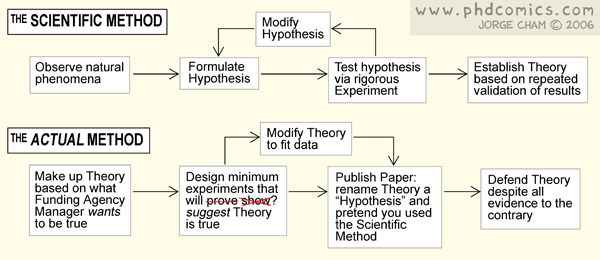
\includegraphics[width=\textwidth]{how-to-do-the-actual-research}
% % \caption{Рекомендации по проведению исследований в рамках диссертации}%
% % \label{fig:how-to-do-research}
% % \end{figure}


% % \Blindtext

% % %%%%%%%%%%%%%%%%%%%%%%%%%%%%%%%%%%%%%%%%%%%%%%%%%%%%%%%%%%%%%%%%%%%%%%%%%%%%%%%%
% % \section{bar}
% % %%%%%%%%%%%%%%%%%%%%%%%%%%%%%%%%%%%%%%%%%%%%%%%%%%%%%%%%%%%%%%%%%%%%%%%%%%%%%%%%

% % \blindtext
% % It is of great importance that you use correct references in your dissertation.
% % Resent studies show that it can increase the chances of successful defense
% % by as much as 3,17 percent~\cite{big,small,russian}.

% % \Blindtext
